\documentclass[a4paper, 12pt]{article}
\usepackage{titling}
\usepackage{array}
\usepackage{booktabs}
\usepackage{enumitem}
\usepackage{graphicx}
\usepackage{hyperref}
\usepackage{amssymb}
\usepackage{listings}
\usepackage{color} %red, green, blue, yellow, cyan, magenta, black, white
\setlength{\heavyrulewidth}{1.5pt}
\setlength{\abovetopsep}{4pt}
\setlength{\parindent}{0pt}
\graphicspath{{.}}

\usepackage[margin=1in]{geometry}
\definecolor{mygreen}{RGB}{28,172,0} % color values Red, Green, Blue
\definecolor{mylilas}{RGB}{170,55,241}
% Must be after geometry
\usepackage{fancyhdr}
\pagestyle{fancy}
\fancyhf{}
\rhead{NN Homework 4}
\lhead{P.Lukin, I. Vishniakou, E. Ovchinnikova}
\cfoot{\thepage}

\setlength{\droptitle}{-5em}

\title{Neural Networks  \\
				- Homework 4 -}
\author{Petr Lukin, Ivan Vishniakou, Evgeniya Ovchinnikova}
\date{Lecture date: 24 October 2016}

\begin{document}

%-------------------------------------------------------------------------------
\lstset{language=Matlab,%
    %basicstyle=\color{red},
    breaklines=true,%
    morekeywords={matlab2tikz},
    keywordstyle=\color{blue},%
    morekeywords=[2]{1}, keywordstyle=[2]{\color{black}},
    identifierstyle=\color{black},%
    stringstyle=\color{mylilas},
    commentstyle=\color{mygreen},%
    showstringspaces=false,%without this there will be a symbol in the places where there is a space
    numbers=left,%
    numberstyle={\tiny \color{black}},% size of the numbers
    numbersep=9pt, % this defines how far the numbers are from the text
    emph=[1]{break},emphstyle=[1]\color{red}, %some words to emphasise
    %emph=[2]{word1,word2}, emphstyle=[2]{style},
}

%-------------------------------------------------------------------------------

\maketitle

\section{Mind map}

\begin{figure}[h]
  \centering
  \caption{Mind map. Chapter 2 (second part) from Haykin’s book.\label{fig:NNstatistical}}
  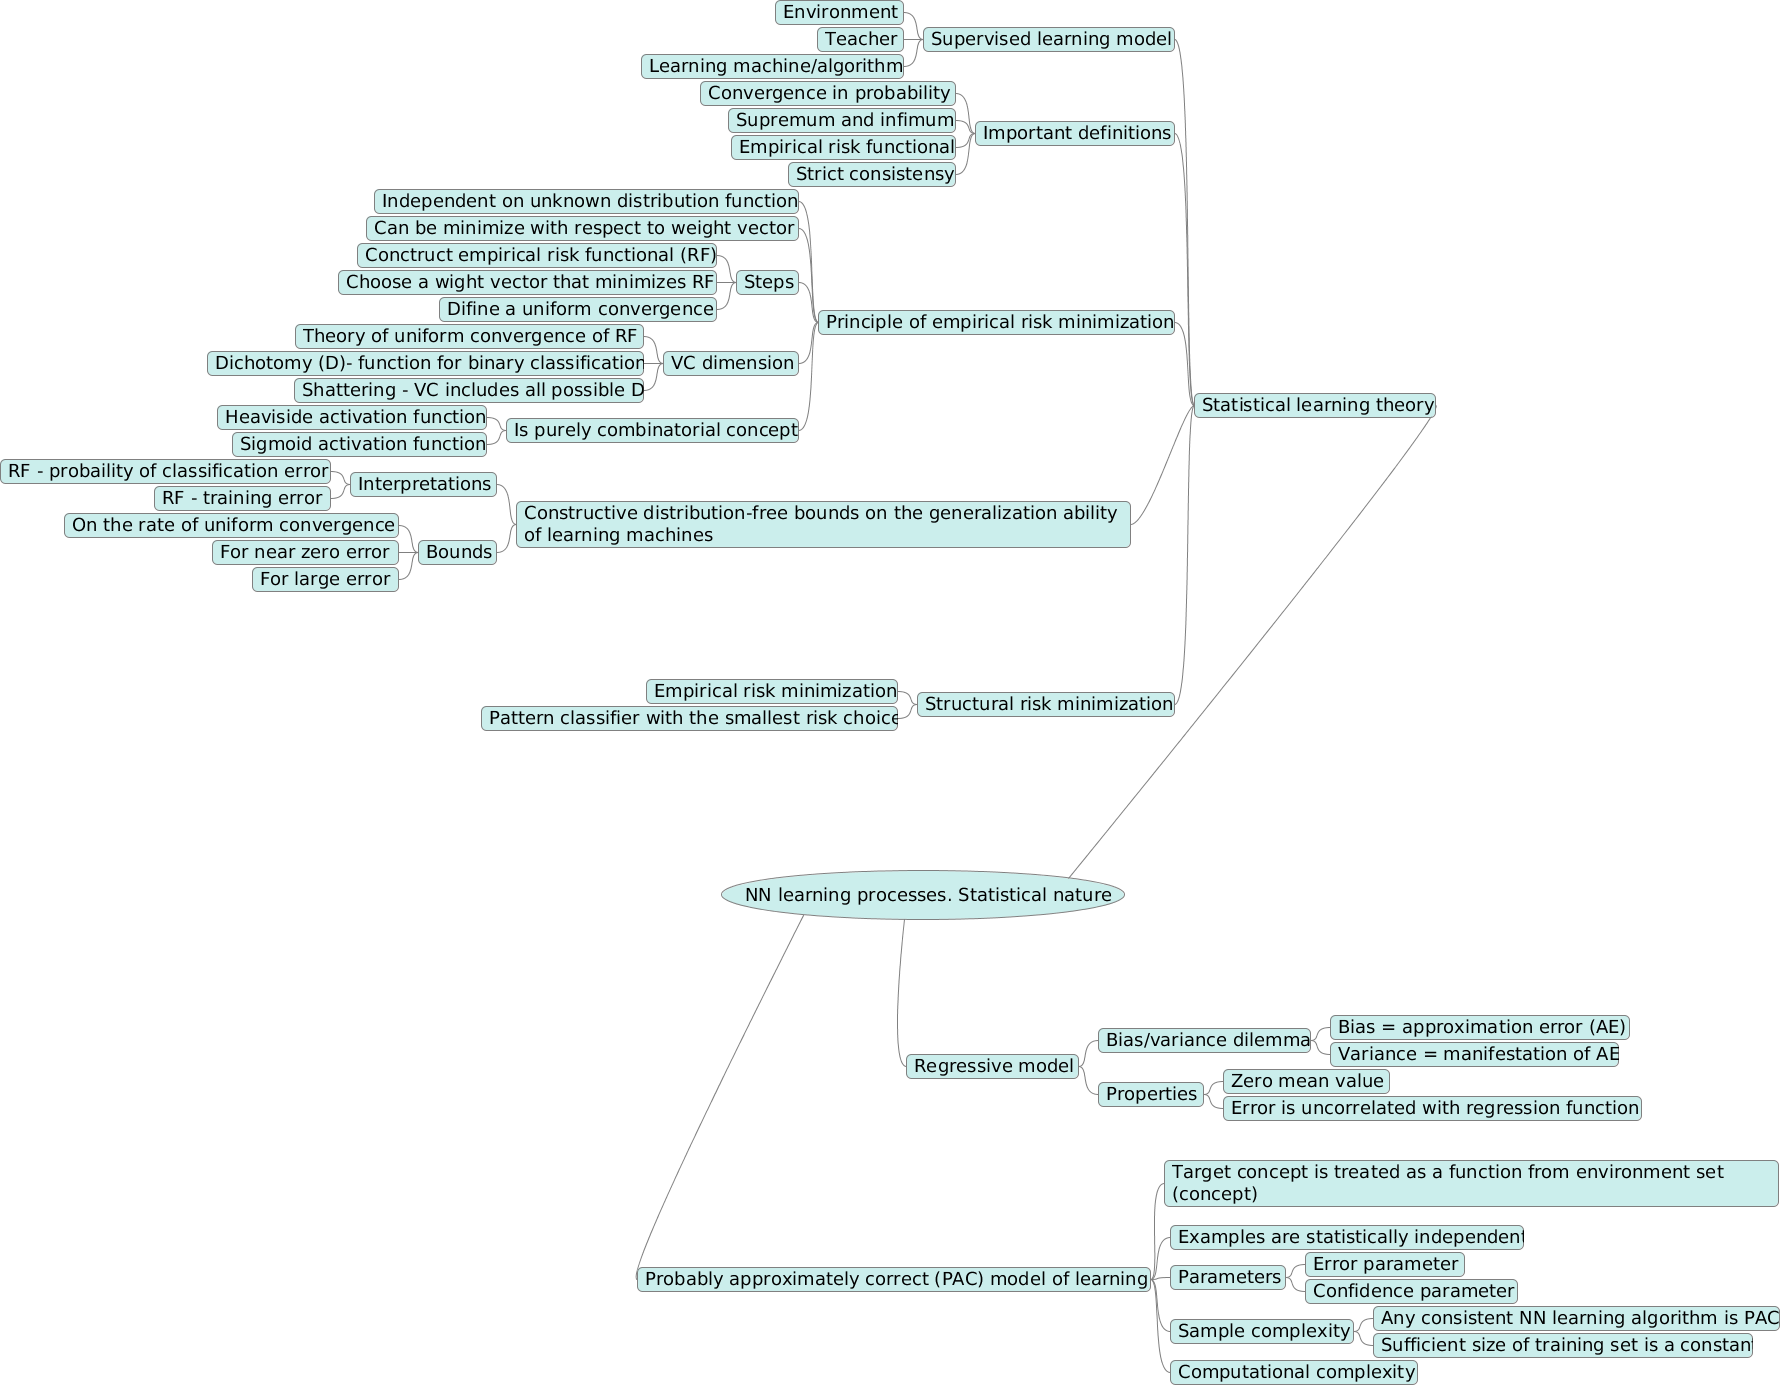
\includegraphics[width=1.0\textwidth]{NNstatistical}
\end{figure}

\section{Exercises}

\subsection*{Exercise 2.1}
Consider the space of instances X corresponding to all points in the x, y plane. Give the VC dimension of the following hypothesis spaces:\\

Solution:\\

a. $H_r$ = the set of all rectangles in the x,y plane. i.e. $H_r = \{((a < x < b) \wedge (c < y < d)) | a, b, c, d \in IR\}$\\

Since $H_r = \{((a < x < b) \wedge (c < y < d)) | a, b, c, d \in IR\}$ we have non-rotatable rectangles only with horizontal and vertical edges those are not tight to the center of coordinate plane. \\
The shattering is possible in case if we can select a certain number of points so it will be possible to choose this number of points minus one without taking into account the last one. In Fig. \ref{fig:RectangularPoints} we show how we can shatter 4 points in all possible combinations. However, we can not choose the five points and select four of them without the fifth one.  Fig. \ref{fig:Rectangular5Points} shows that it is not possible to shatter 5 points. One can see that to define the fifth point we already have four defined points on a rectangle. Fifth point can be either inside or on the edge. Therefore, VC dimension is 4. 

\begin{figure}[h]
  \centering
  \caption{Four points shattered by a rectungular.\label{fig:RectangularPoints}}
  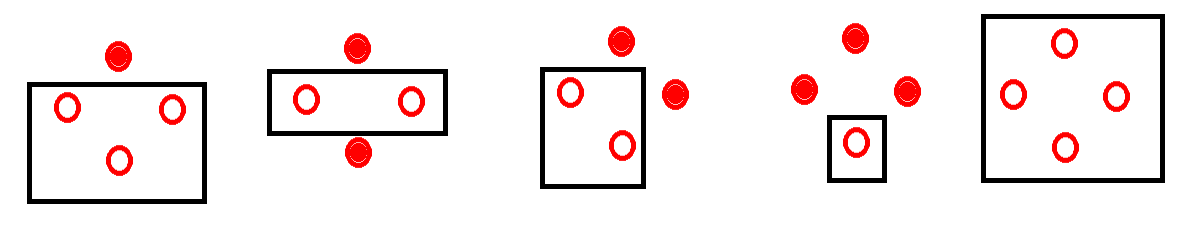
\includegraphics[width=1.0\textwidth]{RectangularPoints}
\end{figure}

\begin{figure}[h]
  \centering
  \caption{Five points not shattered by a rectungular.\label{fig:Rectangular5Points}}
  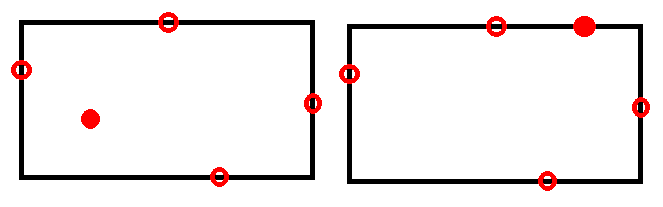
\includegraphics[width=0.6\textwidth]{Rectangular5Points}
\end{figure}


b. $H_c$ = the set of all circles in the x,y plane. Points inside the circle are classified as positive examples.\\

A circle can be defined by 3 points, so the VC is 3. In Fig. \ref{fig:CirclePoints} we show 3 points shattering and in Fig. \ref{fig:Circle5Points} that 4 points cannot be shattered.

\begin{figure}[h]
  \centering
  \caption{Four points shattered by a rectungular.\label{fig:CirclePoints}}
  
\includegraphics[width=0.7\textwidth]{CirclePoints}
\end{figure}

\begin{figure}[h]
  \centering
  \caption{Five points not shattered by a rectungular.\label{fig:Circle5Points}}
  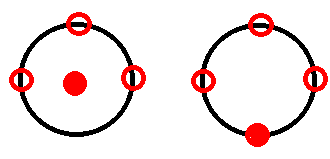
\includegraphics[width=0.5\textwidth]{Circle5Points}
\end{figure}


c. $H_t$ = the set of all triangle in the x,y plane. Points inside the triangle are classified as positive examples.\\

In this case we can always cut 3 points or less of the certain type, because the triangle has three vertices that can be easily seen when we put the points on a circle (see Fig. \ref{fig:TriPoints}). So, it's not a problem to divide 3 from 4 as well as the less number of point and the all cases will be taken into account. In case of 8 points we can only divide 3 points, so the case 4-4 is missing. That is why VC is 7.

\begin{figure}[h]
  \centering
  \caption{Four points shattered by a rectungular.\label{fig:TriPoints}}
  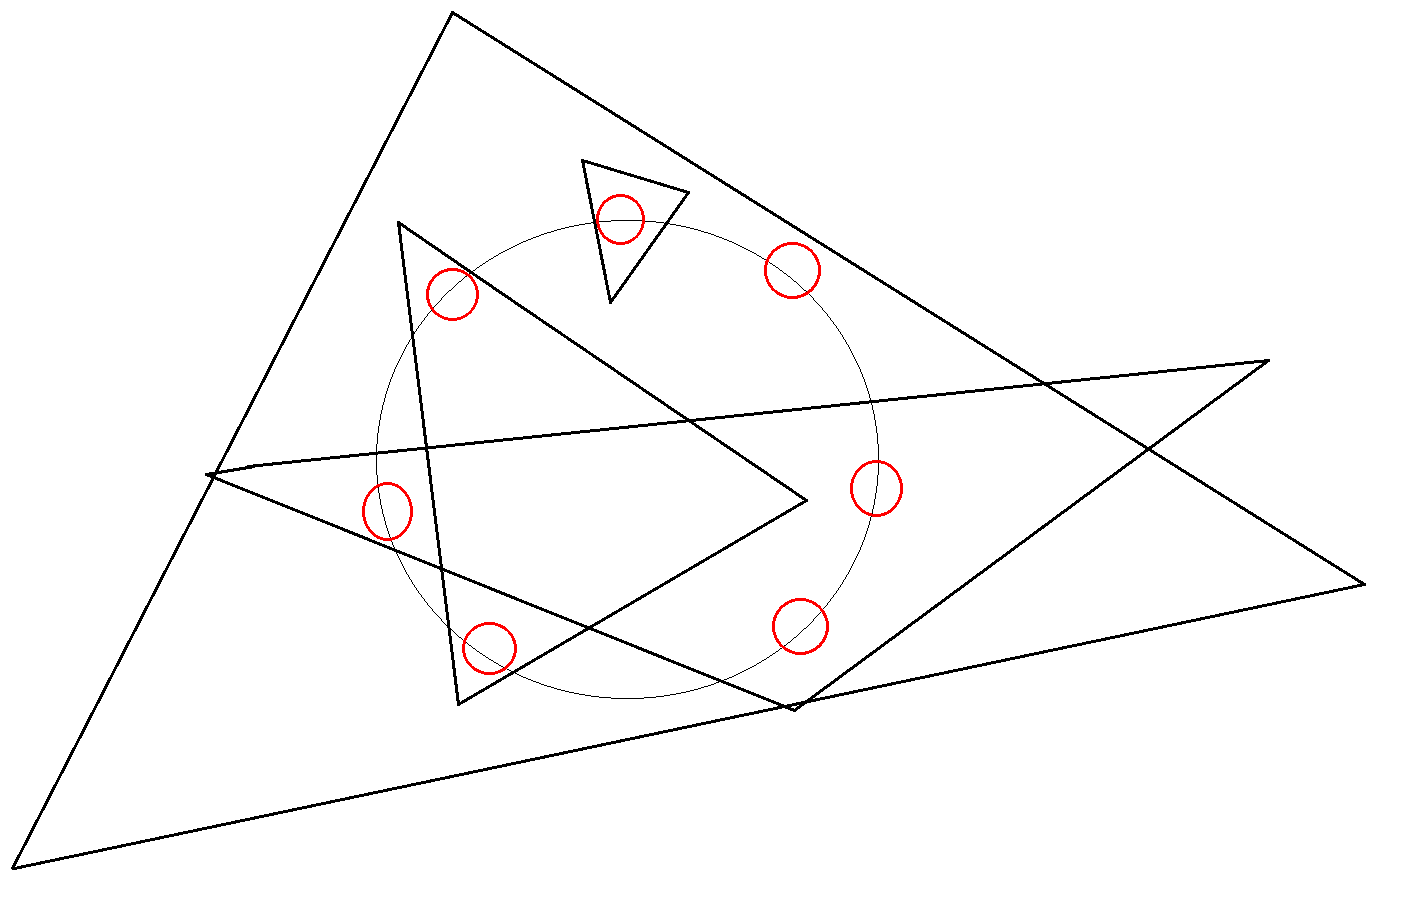
\includegraphics[width=0.7\textwidth]{TriPoints}
\end{figure}

\subsection*{Exercise 2.2}

Definition: consistent learner

\begin{itemize}
\item A learner is consistent if it outputs hypotheses that perfectly fit the training data, whenever possible. It is quite reasonable to ask that a learning algorithm be consistent, given that we typically prefer a hypothesis that fits the training data over one that does not. \\

Task:
\item Write a consistent learner for $H_r$ from last Exercise (i.e. $H_r = \{((a < x < b) \wedge (c < y < d)) | a, b, c, d \in IR\}$ ). Generate a variety of target concept rectangles at random, corresponding to different rectangles in the plane. Generate random examples of each of these target concepts, based on a uniform distribution of instances within the rectangle from (0,0) to (100, 100).

\end{itemize}

Plot the generalization error  as a function of the number of training examples, m. On the same graph, plot the theoretical relationship between e and m, for d = .95. Does theory fit experiment?\\

Solution:\\

Generalization error ($ \hat{\epsilon}\epsilon (h)$) is given as the following:\\

for each sample $Z_i = 1\{ h_i(x) \neq c(x) \}$ (Bernoully random variable):\\

$$\hat{\epsilon} = \frac{1}{m}\sum_{j=1}^{m} Z_i$$

Probability that the version space with respect to $H_r$ and S (a sequence of training examples $m\geqslant 1$ ) is not $\epsilon$-exhausted (with respect to c) is less than $|H| e^{-\epsilon m}$, where  $\epsilon$ is an error. $0<\epsilon<0.5$, probability $0<\delta<0.5$.\\

$\epsilon \geqslant \frac{1}{m}(lnH + ln\frac{1}{\delta})$, so:

$\epsilon \geqslant \frac{1}{m}(ln4 + ln\frac{1}{(1-0.95)})$



\end{document}
